\chapter{Eureka: Motifs are blueprinted communities}
\label{ch:bubbles}

Chapter~\ref{ch:motifs} ended in a state that ought to be uncomfortable. The same
networks, counted by three methods differing only in what they are permitted to
say, gave community counts a hundred apart --- $BB(n,2)$ at $n=6400$ reads
$102$ communities under a nested block model and one under the same model with
squares in its alphabet. Three rules changed limit
class when nothing about them changed but the vocabulary. And the quantity
Chapter~\ref{ch:graphons} had offered as what a locally grown network converges
to --- the density of communities, constant in size and set by the rule --- came
out as one number under a block model and another under a block model that can
name a square. A quantity that moves that far when the describer's vocabulary
changes invites the question whether it was measuring the network at all.

This chapter is the answer, and the answer is not that the disagreement was a
mistake. It is that the two vocabularies were counting the same thing in
different units.

The hypothesis takes one sentence, and the rest of the chapter is what happens
when it is taken seriously. A motif and a community are the same object at two
scales. Both are the description saying \emph{these nodes belong together, and
here is how they are joined}. A motif says it from a blueprint --- a template
fixed in advance, identical in every copy, paid for once and then stamped out
wherever it fits. A community says it bespoke --- a size and an internal density
inferred for that group alone, paid for again for every group. Neither is more
real than the other. They are two ways of buying the same structure, and minimum
description length shops for the cheaper.

Follow that and a good deal of what looked like instability turns into
bookkeeping. A rule whose footprint can be stamped over the whole network needs
no bespoke groups and reports none. A rule whose footprint overlaps itself can be
only partly stamped, and whatever the blueprint cannot cover has to be bought at
the bespoke rate --- which is what a community is. The community count stops
being a property of the network and becomes the size of a remainder. What does
not move is the total.

That is a claim about descriptions rather than about any one network, so testing
it needs a family and not an example: rules that differ in their local structure
and in nothing else, so that the remainder can be made to grow and shrink while
everything around it is held still.

The bubble model is that family, and it is the reason this chapter exists.
$BB(n,L)$ of Chapter~\ref{ch:communities} lays a chain of $L$ new nodes across a
randomly chosen existing link, closing a fresh cycle of length $L+2$; it is the
only rule in this book with a knob that changes the local structure and nothing
else. The reach changes with $L$, and so does the density, but the construction,
the attachment rule and the growth are fixed. Sweeping $L$ from one to five, and
then building two variants of $L=2$ that break the pattern deliberately, puts
rules on both sides of Chapter~\ref{ch:motifs}'s divide and lets us ask what
survives the crossing. The answer, when it comes, is a single number that does
not care which side a rule is on --- but the route to it runs through an
alternation nobody predicted, a lattice that describes itself, and one experiment
whose result was called in advance and came out right.

\section{A dial for the shortest cycle}
\label{sec:bb-dial}

\begin{figure}[t]
  \centering
  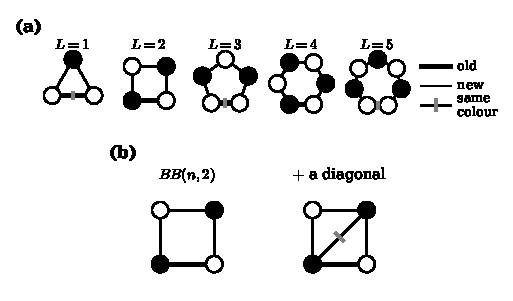
\includegraphics[width=\linewidth]{figs/fig-bb-parity.pdf}
  \caption{\textbf{Two-colouring the $L+2$ cycle.} It closes for even $L$. For
  odd $L$, or for any $L$ once a diagonal is added, one link is left with both
  ends the same colour.}
  \label{fig:bb-parity}
\end{figure}

What $L$ controls is the shortest cycle the rule ever closes, and through it the
whole cycle spectrum. Two faces sharing a link close a cycle of length $a+b-2$,
so the lengths present are generated by the motif and its gluings and everything
else is empty: $BB(n,1)$ carries every length, $BB(n,2)$ carries $4,6,8,10$,
$BB(n,3)$ carries $5$ and $8$, $BB(n,4)$ carries $6$ and $10$. The clustering
coefficient follows the same arithmetic --- $0.74$ at $L=1$ and exactly zero for
every $L$ above it, since no rule but the first closes a triangle.

Chapter~\ref{ch:communities} already measured what the dial does to the onset of
communities, and the answer was not a clean monotone. The Ramsey community number
climbs steeply with $L$, from $108$ at $L=1$ to fifty-six thousand at $L=9$, and
riding on the climb is an alternation: $246$ at $L=3$ against $326$ at $L=2$ and
$2201$ at $L=4$; $752$ at $L=5$ against $2201$ below it and $6595$ above.
\emph{Every} odd $L$ sits beneath both of its even neighbours. Communities come
on sooner when the cycle the rule closes is odd, and that chapter recorded the
effect without explaining it.

The measurements here reproduce it where the grid allows. Fitting the flat
degree-corrected block model on sizes $100,200,400,\ldots$, the onsets come out
at $90$, $400$, $400$, $1600$ and $800$ for $L=1$ to $5$, against the published
$108$, $326$, $246$, $2201$ and $752$. The two middle values collapse onto one
grid point --- $326$ and $246$ are not separable at a spacing of two --- but
$L=4$ against $L=5$ is resolved and comes out the right way round, $1600$ against
$800$, and the $L=5$ figure agrees with the published $752$ to within the grid.
That the odd rules form communities sooner is not an artefact of one
implementation.

\section{Extending the alphabet}
\label{sec:bb-alphabet}

Chapter~\ref{ch:motifs} fitted these networks with an alphabet of the link, the
triangle and the square. Run $BB(n,3)$ through it and the fit plants nothing:
there are no triangles in a pentagon-built network and no squares either, so the
enlarged model costs the price of announcing two totals that turn out to be zero
and buys nothing. Read the output naively and $BB(n,3)$ is a rule whose community
density is untouched by the motif alphabet --- filed alongside
duplication--divergence, in the class where the vocabulary makes no difference.

That reading would be worthless, and the reason is the lesson
Chapter~\ref{ch:motifs} spent itself establishing, turned on the instrument that
established it. A class is a property of a network together with the code used to
describe it. An alphabet with no symbol for a pentagon cannot be asked whether
naming pentagons dissolves communities; it can only report that it has no
pentagons to name. The whole point of the exercise is to give each rule a
vocabulary equal to its own footprint and then see what happens, and for $L>2$
that vocabulary did not exist.

So the alphabet is extended by the cycles above the square. An $L$-cycle has
$|\mathrm{Aut}|=2L$, the dihedral group of $L$ rotations and a reflection, which
is the number Eq.~\eqref{eq:gr-omega} divides by so that one planted copy is
charged once rather than once for every way of writing it down; the convention
checks out, since $k!/|\mathrm{Aut}|=(k-1)!/2$ returns twelve distinct
five-cycles on five labelled nodes, sixty six-cycles on six, and three hundred
and sixty seven-cycles on seven. The triangle and the square keep the
special-cased enumerators they always had, so nothing measured before this family
existed can have moved.

Every rule below is then fitted twice on the same networks: once with the
\emph{control} alphabet of link, triangle and square, which is
Chapter~\ref{ch:motifs}'s and which for $L>2$ has no symbol for the rule's own
cycle, and once with the \emph{test} alphabet, the same plus the $L+2$ cycle.

The control is not decoration. It is the check that the extended fit
reduces to the nested block model when it has nothing to name, and it does: on
$BB(n,3)$ at $n=3200$ the control returns $24.3$ communities against the nested
model's $24.1$. Whatever the test column then reports is the alphabet at work and
not a change of software.

\section{The family}
\label{sec:bb-family}

Seven rules, twenty realisations at each size, exponents fitted from $n=400$
upward so that every rule is past its own onset and none of them contributes a
stretch of $\kappa=1$ to a slope.

\begin{center}
\footnotesize\setlength{\tabcolsep}{3pt}
\begin{tabular}{lccrrrrr}
\hline
rule & cycle & bip. & $\langle k\rangle$ & $r_\kappa$ & $\beta$ nested & $\beta+$mot. & named\\
\hline
$BB(n,1)$ & $3$ & no & $4.00$ & $100$ & $0.89$ & $0.89$ & $54\%$\\
$BB(n,2)$ & $4$ & yes & $3.00$ & $400$ & $0.98$ & --- & $57\%$\\
\quad $+$ a link, bipartite & $4$ & yes & $3.97$ & $100$ & $0.92$ & $0.94$ & $5\%$\\
\quad $+$ a diagonal & $4$ & no & $3.97$ & $100$ & $0.97$ & $0.93$ & $64\%$\\
\hline
$BB(n,3)$ & $5$ & no & $2.67$ & $400$ & $0.95$ & $0.96$ & $55\%$\\
$BB(n,4)$ & $6$ & yes & $2.50$ & $1600$ & $1.07$ & --- & $56\%$\\
$BB(n,5)$ & $7$ & no & $2.40$ & $800$ & $1.05$ & $1.08$ & $54\%$\\
\hline
\end{tabular}
\end{center}


\noindent The exponents in the $\beta$ nested column all sit near one, which is
Chapter~\ref{ch:graphons}'s modular limit: under a nested block model every
member of this family has a constant density of communities. What the alphabet
does to that density is the last two columns, and it alternates.

$L=1$, $3$ and $5$ keep everything. Their exponents are unmoved to within two
hundredths --- $0.89$ against $0.89$, $0.95$ against $0.96$, $1.05$ against
$1.08$ --- while the alphabet works hard the whole way: $BB(n,3)$ plants pentagons
covering fifty-five per cent of its links and saves $2362$ bits at $n=3200$, and
$BB(n,5)$ plants heptagons covering fifty-four per cent and saves a thousand at
$n=1600$. These are not fits in which the enlarged model declined the offer. The
motifs are named, in quantity, at a large and growing saving, and the communities
do not notice.

$L=2$ and $L=4$ lose them. $BB(n,2)$ goes from $44.7$ communities under the
nested model at $n=3200$ to one; $BB(n,4)$ goes from $11.9$ to $2.65$, its
likelihood of finding any communities at all peaking at $0.55$ near $n=800$ and
falling to $0.25$ and $0.15$ at $1600$ and $3200$. Neither carries an exponent in
the table, and for the reason Section~\ref{sec:gr-none} gave for the first of
them: the answer is bimodal, most realisations returning a single community and a
minority returning what the block model returns, so the mean is a mixing ratio
rather than a law.

The pattern is not subtle, and Figure~\ref{fig:bb-alternation}a is the whole of
it. Naming a rule's own motif abolishes its communities when $L$ is even and
leaves them exactly where they were when $L$ is odd.

The figure plots a ratio rather than the two community counts, and the reason is
worth a sentence, because it is the chapter's argument in miniature. These rules
differ several-fold in how many communities they have to begin with --- $BB(n,2)$
has three times $BB(n,4)$'s at the same size --- and that difference is exactly
what does \emph{not} decide the outcome. Dividing it out leaves one quantity per
rule, on a scale where surviving means one, and the five curves separate into two
families that nothing else about them separates.

\begin{figure}[t]
  \centering
  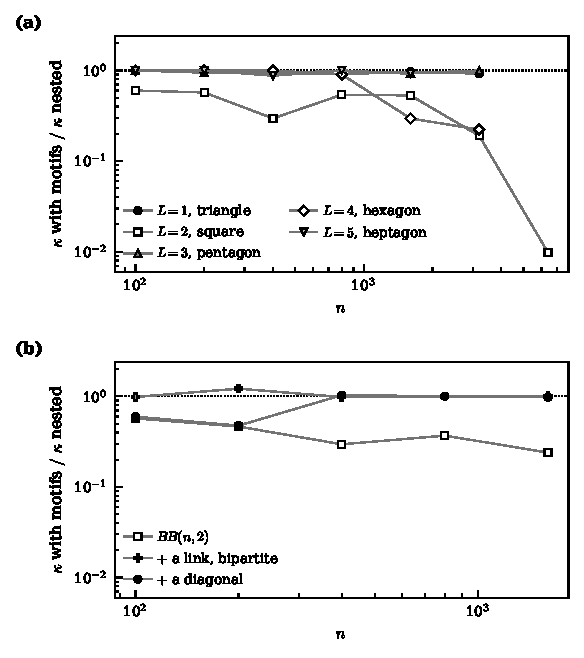
\includegraphics[width=\linewidth]{figs/fig-bb-alternation.pdf}
  \caption{\textbf{The alternation, and the diagonal that breaks it.} Both panels
  plot the community count under the motif alphabet divided by the count the
  nested block model returns on the same networks: one where the communities
  survive, falling away where they are carried off. \textbf{(a)}~$L=1$ to $5$,
  odd $L$ filled and even $L$ open. \textbf{(b)}~$BB(n,2)$ against two variants
  that each add one link per step, of which only the diagonal destroys
  bipartiteness.}
  \label{fig:bb-alternation}
\end{figure}

\section{What does not decide}
\label{sec:bb-negative}

Two explanations were available before this sweep, and the table kills both.

\subsection*{Not how much of the network the motif covers}

Chapter~\ref{ch:motifs} found that on the two deterministic lattices the
discriminator is tiling: the diamond's squares cover ninety-two per cent of its
links and its density dies, the pseudofractal's triangles reach fifty-six and its
density survives. Extended to this family the account predicts that the rules
whose motifs cover more should be the ones that dissolve.

They are not distinguishable at all. The last column reads $54$, $57$, $55$, $56$
and $54$ per cent for $L=1$ to $5$ --- a spread of three points across a family
whose outcomes are opposite. The largest coverage in the whole family belongs to
$BB(n,2)$ at fifty-seven per cent and the smallest to $BB(n,1)$ and $BB(n,5)$ at
fifty-four, and one of those three dissolves while the other two do not. Whatever
tiling explains about the lattices, where the gap is ninety-two against
fifty-six, it explains nothing here.

\subsection*{Not how much there was to lose}

The other candidate was the other side of the ledger. A near-tie in description
length is easiest to reach when the partition was not contributing much in the
first place, and $BB(n,2)$ is a marginal community-former --- a Ramsey number of
$400$ against $BB(n,1)$'s $100$. A rule with thin community structure should be
the one whose communities the alphabet can carry off.

$BB(n,4)$ and $BB(n,5)$ settle that, and they settle it against. At $n=1600$ they
have almost exactly the same amount to lose, $6.10$ communities against $6.85$
under the nested model, and their alphabets name the same share of links, fifty-six
per cent against fifty-four. One collapses to a single community and the other
does not move. If thinness were deciding, the thinner of the two would go first;
$BB(n,5)$ is the thinner by every measure in the table --- fewer communities,
lower mean degree, a later onset than $L=3$ --- and it is the one that survives.

\section{Parity}
\label{sec:bb-parity}

What is left is the one property that has been sitting in plain view since
Section~\ref{sec:bb-dial}. $BB(n,L)$ closes cycles of length $L+2$ and glues
them at shared links, so for even $L$ every cycle in the network is even and the
network is bipartite; for odd $L$ it is not. Two-colouring a grown instance of
each confirms it directly rather than by inference from the cycle spectrum: $L=2$
and $L=4$ two-colour, $L=1$, $3$ and $5$ do not.

The two rules that dissolve are the two that are bipartite. That is the whole of
the regularity, and it holds across five rules whose coverage is constant, whose
community counts vary by a factor of three, and whose mean degrees run from $2.4$
to $4.0$. This is the geometry drawn in Figure~\ref{fig:bb-parity}.


It also connects to something Chapter~\ref{ch:communities} recorded and could not
explain. The alternation in the Ramsey number is the same alternation: every odd
$L$, which is to say every non-bipartite member of the family, forms communities
sooner than either of its even neighbours. So bipartiteness is doing two things
at once in this family --- making communities harder to form in the first place,
and making them easier to argue away once a vocabulary exists that can name the
rule's motif --- and the second was invisible until an alphabet was built that
could reach past the square.

\section{The diagonal}
\label{sec:bb-diagonal}

A regularity across five rules is not a mechanism, and parity in this family is
confounded with everything else $L$ controls. The way to test it is to break
bipartiteness while changing nothing else, and the bubble rule makes that easy,
because a square has diagonals.

Take $BB(n,2)$ and, having laid the chain $u$--$a$--$b$--$v$ across the link
$(u,v)$, add one diagonal. The chain is still two nodes, the reach is unchanged,
one fresh footprint is still laid down per step, and the rule is local in exactly
the sense it was before. But $a$ and $v$ sit on the same side of the bipartition
--- that is what a diagonal of a four-cycle is --- so the added link closes two
triangles and the network stops being bipartite. Parity predicts the communities
survive. Tiling predicts they dissolve, since the footprint still tiles.

The footprint is now $K_4$ minus an edge: four nodes, five links, two triangles
sharing the diagonal, with $|\mathrm{Aut}|=4$ because the two degree-two nodes may
swap and so may the two degree-three nodes, giving $k!/|\mathrm{Aut}|=6$, one for
each choice of the missing link. It has to go into the alphabet, for the reason
of Section~\ref{sec:bb-alphabet} in a subtler form: without it the fit does not
report nothing, it reports the \emph{pieces}. On twenty disjoint copies the
link-only description costs $1820$ bits, the triangle-and-square alphabet $1415$
--- naming each object as a square with one link left over --- and the alphabet
with the symbol $1028$, planting exactly twenty. A rule fitted without the symbol
would have been measured on a description of its footprint's fragments.

Three rules were grown, because the diagonal also adds a link and densification is
the alternative account of anything that moves:

\begin{center}
\footnotesize
\begin{tabular}{llcc}
\hline
rule & extra link per step & $\langle k\rangle$ & bipartite\\
\hline
$BB(n,2)$              & ---                                        & $3.00$ & yes\\
$+$ a link             & to a neighbour of $v$, the opposite colour & $3.97$ & yes\\
$+$ a diagonal         & to $v$, the same colour                    & $3.97$ & no\\
\hline
\end{tabular}
\end{center}

\noindent The result is in the master table, and it is unambiguous. The chorded
rule keeps its communities: from $n=400$ its count is indistinguishable from the
nested model's --- $11.95$ against $11.60$, $23.15$ against $23.05$, $43.25$
against $44.30$ --- with an exponent of $0.93$ against $0.97$. And it keeps them
while the alphabet takes up \emph{more} of it than any other network in this
book: two hundred and ninety-six chorded squares at $n=1600$, sixty-four per cent
of the links named, a saving of $1272$ bits.

That is the tiling account refuted on its own terms. A footprint that covers
sixty-four per cent of the network leaves the communities untouched, while one
covering fifty-seven per cent abolishes them, and the difference between the two
rules is one link per step and the parity it destroys.

Two cautions, because the experiment is not as clean as its result.

The bipartite control did not work. It was built to hold density fixed while
keeping the network two-colourable, and it does that, but the extra link turns
the rule's disjoint squares into overlapping ones and the alphabet is left with
almost nothing it can name --- five per cent of the links, against fifty-seven
without the extra link. Its communities survive, but they survive the way
duplication--divergence's do, because no motif was ever planted, and that says
nothing about parity. A rule that is bipartite, as dense as the chorded one, and
still has separable squares would close the argument; every link that can be
added to a bipartite rule creates overlapping even cycles, and no such rule has
been found.

So density is not controlled within the three rules of this experiment: the only
one that is both bipartite and has an alphabet that engages is $BB(n,2)$ itself,
at $\langle k\rangle=3$. What closes it is the family from outside. Mean degree
runs $4.00$, $3.00$, $2.67$, $2.50$, $2.40$ down the sweep, and the outcome
alternates against that ordering rather than following it: $L=1$ survives at the
highest density in the family and $L=5$ survives at the lowest, with the two
casualties in between. Nothing monotone in $\langle k\rangle$ can produce that.

\section{The same rule, made deterministic}
\label{sec:bb-deterministic}

Everything so far has been measured on a rule that chooses one link at random per
step. Make it deterministic --- lay a chain across \emph{every} link of the
current network, at every generation --- and the family becomes a sequence of
lattices, one network per size, in the way the pseudofractal web and the diamond
lattice are lattices. Call it $DBB(n,L)$.

Two of its members are already in this book under other names. $DBB(n,1)$ hangs
one node on both ends of every link and is exactly the pseudofractal web; it
reproduces $n$ and $m$ at every generation. $DBB(n,2)$ is a cousin of the diamond
lattice rather than the lattice itself --- both quadruple their links each
generation and agree on $n$ and $m$ at every size, but the diamond \emph{replaces}
each link by two parallel paths and leaves its endpoints unjoined, while $DBB$
keeps the link and runs the chain alongside it. The counts follow from the rule:
$m_t=(L+2)^t$, $n_t = 2 + L\big((L+2)^t-1\big)/(L+1)$, and
$\langle k\rangle\to 2(L+1)/L$, the same limiting density as the random family.

Removing the randomness was meant to remove a nuisance. There is one network per
size, nothing to average over, and the alternation --- if it is there --- has to
show up in a single object rather than in a mean. What it removed instead was the
cover the randomness had been providing, and the result is a caution that applies
to Chapter~\ref{ch:motifs} as much as to this one.

\subsection*{Every one of these lattices tiles perfectly}

A generation gives every existing link exactly one chain. So the motifs closed at
the \emph{last} generation have distinct old links and disjoint new chains, and
they use $(L+2)\,m_{t-1}=m_t$ links between them: a perfect edge-disjoint tiling
of the whole network by its own motif, at every size, for every $L$. Counted
directly, $729$ of $729$ triangles on the pseudofractal at $t=7$, $1024$ of
$1024$ squares on $DBB(n,2)$ at $t=6$, $625$ of $625$ pentagons on $DBB(n,3)$ at
$t=5$. The same holds for the diamond lattice.

That is a statement about the networks, proved by construction rather than
fitted. Set against it, what the fit reports is a statement about the search:

\begin{center}
\footnotesize\setlength{\tabcolsep}{4pt}
\begin{tabular}{lrrrr@{\hskip 10pt}rrr}
\hline
 & & \multicolumn{3}{c}{as fitted} & \multicolumn{3}{c}{seeded from the tiling}\\
lattice & $n$ & $\Sigma$ & $\kappa$ & named & $\Sigma$ & $\kappa$ & named\\
\hline
pseudofractal & $366$   & $4\,724$  & $3$  & $45\%$ & $\mathbf{3\,887}$  & $1$ & $100\%$\\
pseudofractal & $1\,095$ & $15\,487$ & $16$ & $56\%$ & $\mathbf{13\,728}$ & $1$ & $100\%$\\
$DBB(n,2)$    & $684$   & $8\,459$  & $1$  & $66\%$ & $\mathbf{7\,434}$  & $1$ & $100\%$\\
$DBB(n,2)$    & $2\,732$ & $42\,837$ & $26$ & $13\%$ & $\mathbf{35\,666}$ & $1$ & $100\%$\\
diamond       & $684$   & $7\,812$  & $3$  & $88\%$ & $\mathbf{7\,434}$  & $1$ & $100\%$\\
diamond       & $2\,732$ & $37\,213$ & $5$  & $88\%$ & $\mathbf{35\,666}$ & $1$ & $100\%$\\
\hline
\end{tabular}
\end{center}

\noindent The right-hand columns are the known tiling handed to the optimiser as
a starting state and allowed to move. It does not move: it stays on the tiling,
and the description is cheaper than the fitted one every time, by $378$ bits at
the smallest and $7172$ at the largest. So on the criterion this book uses
throughout, the best available description of the pseudofractal web has
\emph{one} community, not the sixteen the fit reports at $n=1095$ --- and the same
is true of the diamond.

Two of those rows have the same description length to the bit, $7434$ at $n=684$
and $35\,666$ at $n=2732$, because $DBB(n,2)$ and the diamond are both tiled by
squares on the same $n$ and $m$. Two lattices that Chapter~\ref{ch:motifs} placed
in different limit classes are, under their best descriptions, indistinguishable.

\subsection*{The same thing happens all the way up the family}

Section~\ref{sec:gr-square} makes this argument for the two lattices
Chapter~\ref{ch:motifs} fits, and finds that both of them have one community
under their best description rather than the fourteen and the seven the search
reports. What the sweep adds is that it is not a peculiarity of those two. It is
what every deterministic member of this family does, at every $L$, for a reason
that is written into the rule: give every link a motif at every generation and
the last generation's motifs are a tiling, whatever the motif is.

So the parity that organises the random family has nothing to organise here.
$DBB(n,L)$ is in the first class for every $L$ measured, odd and even alike, and
the alternation of Sections~\ref{sec:bb-family} to \ref{sec:bb-diagonal} is a
fact about rules that choose one link at a time.

\subsection*{Why the random family is not touched}

The randomness is what makes $BB(n,L)$ measurable. Its motifs are laid across
links chosen at random, so they overlap: a link that has already been built into
one motif can be chosen again, and no perfect tiling exists to be missed. The
fifty-four to fifty-seven per cent the alphabet names there is close to what is
available, not a sixth of it, and it is stable across sizes and realisations
rather than collapsing as the network grows. That is why the alternation of
Sections~\ref{sec:bb-family} to \ref{sec:bb-diagonal} is a measurement and this
section is a caution.

It is worth saying plainly which way that cuts. A deterministic rule looks like
the cleaner instrument --- no sampling, no averaging, one object per size --- and
it is the one on which the instrument fails. Stochasticity is not noise obscuring
the structure here. It is what keeps the structure within reach of a greedy
search, by ensuring there is no exact optimum to be exactly missed.

\section{Motifs are blueprinted communities}
\label{sec:bb-meso}

There is a way of reading this whole chapter that makes the alternation less
strange, and it is worth stating because it also says what the two vocabularies
have been arguing about.

A planted motif and a community are the same kind of object at two scales. Both
are the description saying \emph{these nodes belong together, and here is how
they are joined}. A motif is small, fixed and homogeneous: a handful of nodes, a
wiring given once by the symbol, every copy identical. A community is large,
variable and heterogeneous: as many nodes as the fit wants, an internal density
given by a row of the count matrix, no two alike. Community detection, put this
way, is the representation of a network by heterogeneous motifs of unbounded size
and arbitrary internal connectivity, and an alphabet of motifs is the same
representation with the size fixed and the wiring named in advance.

That is why the two compete. They are not a structure and a description of it;
they are two dialects for the same statement about the same links, and minimum
description length is choosing between dialects. Which is also why "the alphabet
abolished the communities" was always a slightly misleading way to put it. The
meso-structure did not go anywhere. It was renamed.

The counts say so, and they read more easily if the notation admits the point.
Write $\kappa_0$ for the number of motifs the fit plants, against $\kappa$ for the
number of communities it reports: a motif is the null case of a community, the
simplest form the thing can take, fixed in size and homogeneous in wiring, and
the index says so. Follow both along the family (Figure~\ref{fig:bb-meso}):

\begin{center}
\footnotesize
\begin{tabular}{lrrr}
\hline
rule & $\beta$ for $\kappa_0$ & $\beta$ for $\kappa$ & $\beta$ for $\kappa_0+\kappa$\\
\hline
$BB(n,1)$ & $1.06$ & $0.89$ & $1.04$\\
$BB(n,2)$ & $1.02$ & $\mathbf{0.25}$ & $1.01$\\
$BB(n,3)$ & $0.99$ & $0.93$ & $0.99$\\
$BB(n,4)$ & $1.01$ & $\mathbf{0.28}$ & $0.99$\\
$BB(n,5)$ & $1.00$ & $0.70$ & $0.98$\\
\hline
\end{tabular}
\end{center}

\noindent The middle column is the alternation this chapter has been about,
running from $n^{0.25}$ to $n^{0.93}$ with the parity of $L$. The outer two do
not alternate at all. Every rule in the family plants motifs in proportion to its
size, and every rule carries meso-structure in proportion to its size, with a
slope of one to within a few hundredths in all ten cases.

The two panels of Figure~\ref{fig:bb-meso} are nearly the same picture, and that
is the point rather than a defect of it: $\kappa$ is a few per cent of $\kappa_0+\kappa$
throughout, so the total is dominated by the motifs and the communities are a
small residue. What the parity of $L$ decides is the size of that residue --- how
much of the meso-structure is left over for the heterogeneous vocabulary once the
homogeneous one has taken what it can.

\begin{figure}[t]
  \centering
  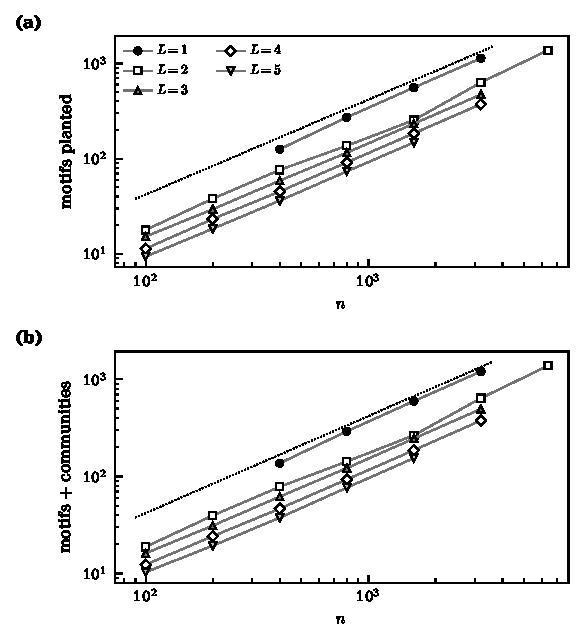
\includegraphics[width=\linewidth]{figs/fig-bb-meso.pdf}
  \caption{\textbf{Meso-structure, counted without regard to which vocabulary
  names it.} \textbf{(a)}~motifs planted, $\kappa_0$, and \textbf{(b)}~motifs plus
  communities, $\kappa_0+\kappa$, against size, with a line of slope one for the
  eye. Every rule is parallel to it in both panels, while $\kappa$ alone runs
  from $n^{0.25}$ to $n^{0.93}$ across the same five rules.}
  \label{fig:bb-meso}
\end{figure}

The density of that meso-structure is a constant of the rule, in exactly the
sense Chapter~\ref{ch:graphons} gave the density of communities: $0.38$ per node
for $L=1$, then $0.20$, $0.15$, $0.12$ and $0.09$ as the motif grows and fewer of
them fit. It falls with $L$ for a reason with no depth in it --- a longer cycle
uses more links per copy, and the mean degree is falling too --- but it is
constant in $n$ for each rule, which is the part that matters.

So Chapter~\ref{ch:graphons}'s conjecture can be restated in a form the diamond
does not break. What a locally grown network converges to is a constant density
of meso-structure. Whether a given description spends that density on motifs or
on communities is a question about the vocabulary, and the answer alternates with
the parity of the cycle; the density itself does not notice. Read that way,
$BB(n,2)$ and the diamond never lost anything. They were re-described, in a
dialect that happens to have a symbol for what they are made of.

\section{What four chapters add up to}
\label{sec:bb-conclusion}

This is the end of four chapters rather than of one, and the accounting is worth
doing in one place. Chapter~\ref{ch:communities} asked whether locally grown
networks have communities and found that they do, with a threshold size and an
exactly solvable case to show why. Chapter~\ref{ch:graphons} asked how many, and
found that the answer moved by four tenths in the exponent when the prior
changed. Chapter~\ref{ch:motifs} asked what the describer is allowed to
\emph{name}, and found that the answer could move by everything: a vocabulary
that can call a set of links a triangle sometimes reports no communities at all
where a vocabulary that cannot reports a constant density of them. This chapter
turned the one dial that changes a rule's local structure and nothing else.

Four chapters of numbers that disagree with each other invites the reading that
none of them means anything. The opposite is the case, and the last section says
why: they disagree because they are counting the same substance in two
currencies. Count it in one.

\begin{center}
\footnotesize\setlength{\tabcolsep}{5pt}
\begin{tabular}{llrr}
\hline
rule & motif & links named & $\beta$ for $\kappa_0+\kappa$\\
\hline
\multicolumn{4}{l}{\emph{no communities}}\\
\quad $BB(n,2)$ & \ngon{4} & $57\%$ & $\mathbf{1.01}$\\
\quad $BB(n,4)$ & \ngon{6} & $56\%$ & $\mathbf{0.99}$\\
\quad pseudofractal & \ngon{3} & $100\%$ & $\mathbf{1.00}$\\
\quad diamond & \ngon{4} & $100\%$ & $\mathbf{1.00}$\\
\hline
\multicolumn{4}{l}{\emph{constant density of communities}}\\
\quad $LS(n,1)$ & \ngon{3} & $62\%$ & $\mathbf{1.01}$\\
\quad $BB(n,1)$ & \ngon{3} & $54\%$ & $\mathbf{1.04}$\\
\quad $BB(n,3)$ & \ngon{5} & $55\%$ & $\mathbf{0.99}$\\
\quad $BB(n,5)$ & \ngon{7} & $54\%$ & $\mathbf{0.98}$\\
\quad $DS(n,1/3)$ & \ngon{4} & $26\%$ & $\mathbf{1.11}$\\
\quad $DS(n,0.5)$ & \ngon{4} & $12\%$ & $\mathbf{1.21}$\\
\quad $DD(n,0.5)$ & $K_{2,d}$ & $0\%$ & $\mathbf{1.11}$\\
\quad $BB(n,2)+$ a link & \sqstub & $5\%$ & $\mathbf{1.10}$\\
\quad $BB(n,2)+$ a diagonal & \sqdiag & $64\%$ & $\mathbf{0.94}$\\
\hline
\end{tabular}
\end{center}


\noindent Thirteen local rules, every one measured in this book, sorted into the
two limits they converge to under the best description available, and one
exponent. The exponent does not sort. It sits on one --- between $0.94$ and
$1.21$, and within a few hundredths of one wherever the alphabet engages at
all --- on both sides of a division that was supposed to separate a network with
communities from a network without any.

\subsection*{Two classes, and what actually separates them}

The classes are real. In the first, the best description uses a single group at
any size: the network is made of copies of one small object, laid down where the
rule put them, and once they are named there is nothing left for a partition to
say. In the second, naming the motifs leaves a residue that only heterogeneous
groups of unbounded size can describe, and the number of those groups grows in
proportion to the network.

What separates them is not how much meso-structure a rule builds. It is whether
the rule's own footprint can be laid down over the whole network without
overlapping itself. Where it can --- exactly, in the two lattices, which tile
themselves; nearly, in $BB(n,2)$ and $BB(n,4)$, whose fresh cycles land on new
nodes --- the blueprint suffices and the communities go. Where the footprints
pile onto each other, as duplication's bicliques do at nought per cent and local
search's triangles do at sixty-two, a decomposition that gives each link to one
motif cannot take up the network, and the leftover is what a community is.

That is the sense in which a motif is a blueprinted community. Both say
\emph{these nodes belong together, and here is how they are joined}. A motif says
it from a template fixed in advance, identical in every copy, and pays for the
template once. A community says it bespoke, with a size and an internal density
inferred for each one, and pays for every group separately. Minimum description
length is not choosing between structure and no structure. It is choosing how
much of the network can be described from a blueprint, and billing the remainder
at the bespoke rate.

\subsection*{The limit, restated}

Chapter~\ref{ch:graphons} conjectured that a locally grown network converges to
no kernel on the unit square, and that what characterises its limit is intensive:
the density of communities $b=B/n$, constant in size and set by the rule. The
diamond then broke it, and the repair is one substitution. The intensive quantity
is the density of \emph{meso-structure}, $(\kappa_0+\kappa)/n$, and it is
constant for every local rule in the table. The density of communities is
constant only for those in the second class, and zero for those in the first,
because $b$ measures how much of the meso-structure happened to need the
expensive vocabulary.

Read that way the two classes stop being a taxonomy of networks and become a
statement about compressibility. A rule in the first class builds a network that
is wholly blueprinted: one symbol, repeated, with no remainder. A rule in the
second builds one that is partly blueprinted, with a remainder that scales.
Nothing in either case converges to a shape one could draw on the unit square,
and the reason is the one Chapter~\ref{ch:graphons} gave --- the structure never
coarsens, because the rule keeps writing it at whatever scale the network has
reached --- but what fails to coarsen is now countable, and it is the same
quantity in both classes.

\subsection*{What the inference costs}

The other thing these chapters have between them established is how much of a
community count belongs to the counter. Three knobs, and each was found by
turning it and watching:

\emph{Resolution.} The flat block model cannot report more than about $\sqrt n$
groups. Chapter~\ref{ch:communities}'s $0.61$ was that ceiling as much as it was
the networks; the nested prior lifts it and the exponent goes to one.

\emph{Vocabulary.} What the model may name decides what it must partition. Give
it the rule's own motif and three of the eight rules in Chapter~\ref{ch:motifs}
leave the constant-density class outright.

\emph{Search.} The one this chapter had to learn the hard way. On the two
lattices whose optimal description can be written down by hand, the greedy fit
misses it by up to a tenth of the whole description length, and reports a
partition it does not need. Every published number here is a statement about a
network, a code, \emph{and} an optimiser, and only the first two are usually
declared.

The invariant survives all three. Whatever the resolution, whatever the alphabet,
whatever the search finds, the meso-structure comes out proportional to $n$.

\subsection*{Not settled}

Three things, and they are the obvious next measurements rather than
reservations.

Why parity decides the random family is not established. The story --- that a
square is what a bipartite network is made of, so on the even rules the alphabet
and the partition describe the same structure and either can stand in for the
other --- is plausible and untested. A chorded hexagon rule would test it: if
parity is the mechanism, $BB(n,4)$ with a diagonal should keep its communities
exactly as $BB(n,2)$ with one does.

Whether the meso-structure density is constant beyond this book's rules is
unmeasured. Every entry in the table is a growth rule whose construction is
known. The three real growing networks of Chapter~\ref{ch:graphons} are where to
take it, and the fit is within reach for two of them.

And whether the first class contains anything real is open. Its members here are
all lattices or near-lattices, built to tile; no real network is likely to be a
perfect blueprint of one motif. What a real network might plausibly be is a
member of the second class with an unusually large blueprinted fraction, and that
is a quantity this machinery can measure --- the last column of the table --- on
any network one can fit.

One last observation, which belongs to the book's argument rather than to this
family. Every result in this chapter required an alphabet that did not exist when
the chapter began. $BB(n,3)$ fitted with Chapter~\ref{ch:motifs}'s vocabulary
returns a clean, publishable, entirely misleading answer --- no motifs planted,
density untouched, filed with the rules the alphabet cannot reach. The finding
was not hiding in the data waiting to be noticed. It was unreachable until the
instrument was rebuilt, and the instrument was only rebuilt because a conjecture
about the family made a specific enough claim to be worth the trouble. A limit
class is a property of a network together with the code used to describe it, and
these four chapters are what that sentence costs when it is taken seriously.

There is one more thing to say about the density of meso-structure, and it comes from
outside every instrument used here. Everything in these four chapters is an argument
about descriptions --- what a code costs, which vocabulary is cheaper, what a fit is
permitted to name --- so the fair objection is that the invariant might be a property
of the describing rather than of the network. Chapter~\ref{ch:quantum} measures it a
different way. A quantum walker on these networks knows nothing of priors or alphabets
and cannot fit anything; it can only move, and how far it gets is set by the density of
meso-structure and not by whether a statistician would have called that structure a
motif or a community. Two routes this unlike arriving at the same quantity is the best
evidence in the book that it is a thing.
